\section{Time-to-accuracy over $N$, $h$, and $\epsilon$}
\label{sec:tta}

\subsection{The existing statistic underestimates retry cost}
\label{sec:tte-issue}

The source report's crossing statistic (Eq.~\eqref{eq:rollingmean}) is converted into a $99\%$-confidence time-to-solution by treating an unsuccessful seed as a full restart at the median successful time:
\begin{equation}
\mathrm{TTE}_{99}=
\begin{cases}
T_r, & p=1,\\[2pt]
T_r\,\dfrac{\ln(0.01)}{\ln(1-p)}, & 0<p<1,
\end{cases}
\label{eq:tte99}
\end{equation}
implemented exactly this way in \texttt{scripts/viz/paper\_figures.py}, function \texttt{tte99\_from\_validated()} (lines 148--174): a failed seed is simply excluded from the set whose median defines $T_r$ and is accounted for only through $p$. This is the standard retry formula for attempts of a \emph{fixed} runtime, but here a successful attempt can stop early at $t^\star$ while an unsuccessful one consumes the full $100$-iteration budget, and $T_r$ is computed only from the (generally shorter) successful attempts -- so the formula omits the cost of the failed full-budget runs it is nominally accounting for. This matters exactly where the reported crossover is claimed: at $N=64$, the reported successful fractions are FPGA $19/20$, Zephyr(+CEM) $19/20$, SA $18/20$, Metropolis $17/20$, Gibbs $16/20$, so between one and four unsuccessful seeds enter the ranking through $p$ alone. Exact binomial 95\% intervals at these counts are wide (e.g.\ $19/20\Rightarrow p\in[0.751,0.999]$), so the sharp distinction the current formula draws between, say, a $20/20$ and a $19/20$ series is not statistically supported by the underlying counts.

\missing{\textbf{Survival-corrected TTE statistic.} None of a fixed-cutoff estimator ($p_\tau=\Pr(T\le\tau)$, $T_{99}(\tau)=\tau\ln(0.01)/\ln(1-p_\tau)$, minimized over a pre-specified grid of $\tau$ with bootstrap CIs), a Kaplan--Meier / right-censored treatment of $t^\star$, or a full retry-process simulation from the empirical distribution of successes and full-budget failures is implemented anywhere in the audited repository (Sec.~\ref{sec:code-gaps}, item T3). Reproducing Fig.~\ref{fig:tte-corrected} [PLACEHOLDER] with one of these three estimators, re-run on the archived per-seed histories (no new device time required), is the single highest-priority numerical fix in this paper.}

\subsection{Criterion dependence: $\epsilon$ and $h$}
\label{sec:eps-h}

The reported crossover uses a single cell: the 1D TFIM at $h=0.5$ with $\epsilon=0.1$ per spin (a total-energy tolerance of $6.4$ at $N=64$). The target distribution changes qualitatively across $h$ -- strongly peaked in the ordered phase, approaching uniform at large field -- so a result at $h=0.5$ is not presumptively representative of the critical or paramagnetic regime. A sweep over $h\in\{0.5,0.7,0.9,1.0,1.1,1.3,1.5\}$ at fixed $N=16$ already exists in code, \texttt{fig\_tte\_vs\_h\_n16()} in \texttt{scripts/viz/paper\_figures.py} (lines 1469--1541), but it is defined and never invoked -- it does not run as part of the current figure-generation pipeline, and it fixes $\epsilon=0.1$ rather than sweeping it. No script anywhere sweeps $\epsilon$ (every figure function hardcodes a single value, $0.1$ for the validated-convergence figures and $0.01$ for the unrelated ITE figures).

\missing{\textbf{Joint $(\epsilon,h)$ time-to-accuracy grid.} Producing Fig.~\ref{fig:tta-grid} [PLACEHOLDER] -- time-to-accuracy curves for $\epsilon\in\{0.1,0.05,0.02,0.01\}$ at $h\in\{0.5,1.0,2.0\}$, or the lower envelope of wall time vs.\ independently evaluated error suggested by the evaluation -- requires: (i) wiring \texttt{fig\_tte\_vs\_h\_n16()} into the run pipeline and generalizing it to also loop over $\epsilon$; (ii) at $N=64$ specifically, re-deriving each crossing from the independent evaluator of Sec.~\ref{sec:validation} rather than the training log, since this is exactly the size and field at which the current crossover claim (Sec.~\ref{sec:limitations}) is made. Only new QPU time is required at cells not already covered by archived checkpoints.}

Figure~\ref{fig:tte-baseline} reproduces the single existing $(\epsilon,h)=(0.1,0.5)$ cell, labelled explicitly as one point in a criterion space rather than as the general result.

\begin{figure}[t]
\centering
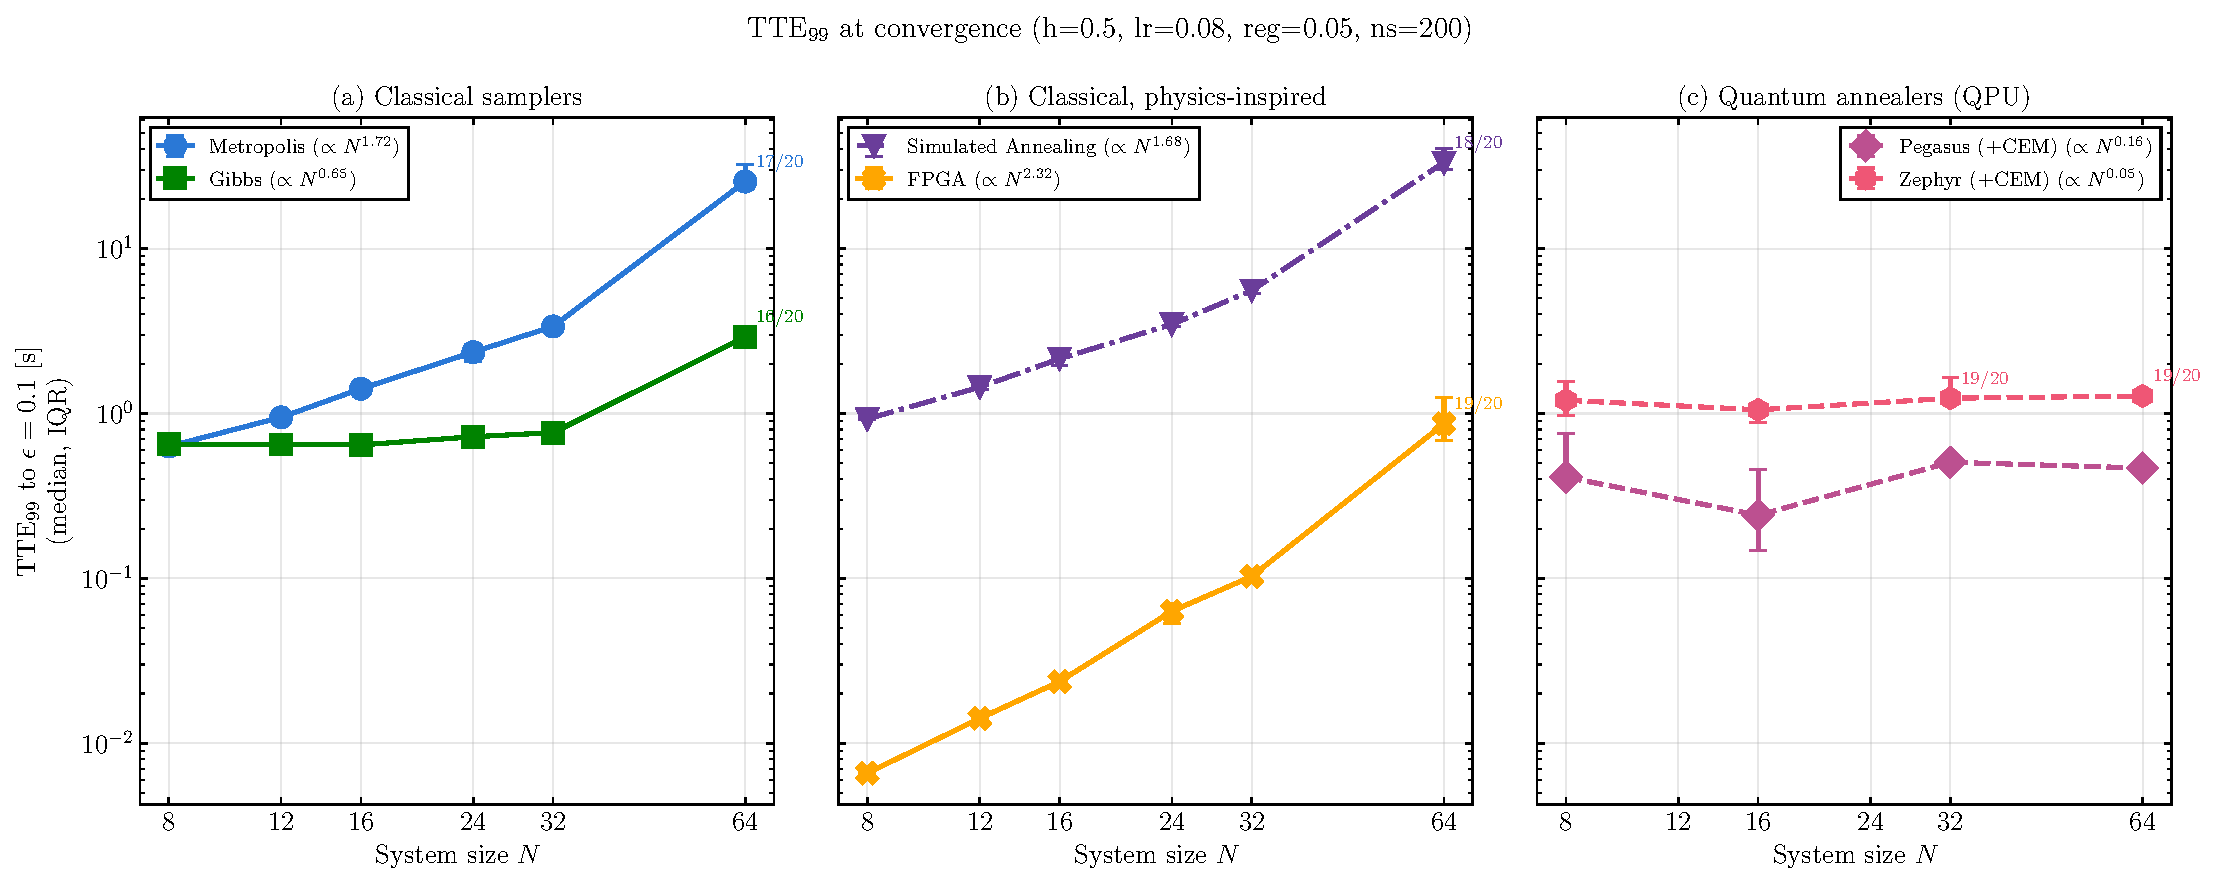
\includegraphics[width=\linewidth]{figures/fig10c_tte99_vs_n_eps0.1.pdf}
\caption{$\mathrm{TTE}_{99}$ (Eq.~\eqref{eq:tte99}) vs.\ $N$ at the single tested cell $h=0.5$, $\epsilon=0.1$. Annotated fractions give the successful-seed count where below $20/20$. This is the only $(\epsilon,h)$ cell for which a full-$N$ curve currently exists; Sec.~\ref{sec:eps-h} explains why it should not be read as representative.}
\label{fig:tte-baseline}
\end{figure}

\subsection{Fixed-protocol vs.\ solver-optimized comparison}

The classical baselines are matched on outer SR settings but not on inner sampling effort: Metropolis restarts with 200 warm-up sweeps plus one sampling sweep, persistent Gibbs uses ten block sweeps after a one-time initialization, and simulated annealing uses 200 warm-up plus 40 cooling sweeps. This fixed-protocol comparison is scientifically useful on its own terms but is not the best-achievable time-to-accuracy of each sampler; sampling-quality figures elsewhere in this project (Fig.~\ref{fig:classical}) show simulated-annealing quality still improving well past 40 sweeps. \missing{\textbf{Solver-optimized comparison.} A second benchmark in which every classical sampler receives the same hyperparameter-tuning budget and independently minimizes its own time-to-accuracy, rather than sharing the outer protocol, is not implemented and is listed as a distinct experiment rather than an edit to the existing one.}
